% Yao: wire keys and garbled gates (1371 x 903 px); the garbled-circuit drawing is a crop
\figsetup{1371}{903}%
\begin{tikzpicture}[fig]
\figbbox
\node[at base] at (87,105) {\fs{50}$\bullet$};
\node[at base] at (148,105) {\fs{50}\fit{785}{Each wire w has 0-key and 1-key}};
\node[at base] at (177,171) {\fs{42}--};
\node[at base] at (229,171) {\fs{42}\fit{758}{Colored ``blue'' and ``green'' at random}};
\node[at base] at (1010,148) {\fs{32}1-key};
\pxkey{1167}{80}{40}{kgreen}{W}
\node[at base] at (1001,354) {\fs{32}0-key};
\pxkey{1160}{278}{42}{kblue}{W}
\node[at base] at (87,309) {\fs{50}$\bullet$};
\node[at base] at (148,309) {\fs{50}\fit{578}{K\textsubscript{i,b}= b-key of input wire i}};
\node[at base] at (87,388) {\fs{50}$\bullet$};
\node[at base] at (148,388) {\fs{50}\fit{790}{g\textsubscript{0}(r) = color code for output wires}};
\node[at base] at (262,465) {\fs{50}\fit{408}{+ ``garbled gates''}};
% plain circuit with wire values
\newcommand{\gate}[4]{\filldraw[fill=cyan!15, draw=black, px=2] (#1,#2) -- (#1+#3,#2) arc[start angle=0, end angle=-180, x radius=#3/2, y radius=#4];
  \filldraw[fill=white, draw=black, px=2] (#1+#3/2,#2-#4-5) circle (5);}
\draw[px=2] (210,785) -- (210,828) (275,785) -- (275,828) (365,785) -- (365,828) (430,785) -- (430,828);
\draw[px=2] (243,738) -- (243,700) -- (290,700) -- (290,678);
\draw[px=2] (397,738) -- (397,712) -- (455,712) -- (455,595);
\draw[px=2] (328,640) -- (328,615) -- (395,615) -- (395,595);
\draw[px=2] (350,678) -- (350,712) -- (397,712);
\draw[arr={2}{10}{8}] (422,550) -- (422,522);
\gate{193}{785}{99}{36} \gate{346}{785}{101}{36} \gate{277}{678}{103}{32} \gate{375}{595}{95}{34}
\node[at base] at (420,525) {\fs{32}\sbf{0}};
\node[at base] at (305,635) {\fs{32}\sbf{0}};
\node[at base, red] at (240,715) {\fs{32}\sbf{0}};
\node[at base] at (405,708) {\fs{32}\sbf{1}};
\foreach \x/\v in {204/0,265/1,370/0,433/0} {\node[at base, red] at (\x,850) {\fs{32}\sbf{\v}};}
\node[anchor=north west] at (795,497) {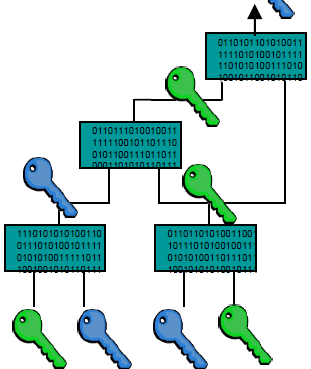
\includegraphics[width=311\fu]{figures/chapter-6-yao-wire-keys-garbled.png}};
\end{tikzpicture}%
